\documentclass[10pt,a4paper]{ctexart}
\usepackage[margin=1.6cm]{geometry}
\usepackage{graphicx,xcolor,hyperref}
\hypersetup{pdftitle={手部与6D：三页配图预览}}
\setlength{\parindent}{0pt}\setlength{\parskip}{6pt}
\pagestyle{plain}
\begin{document}
\begin{center}{\Large\bfseries 手部姿态：原理图与真人演示}\end{center}
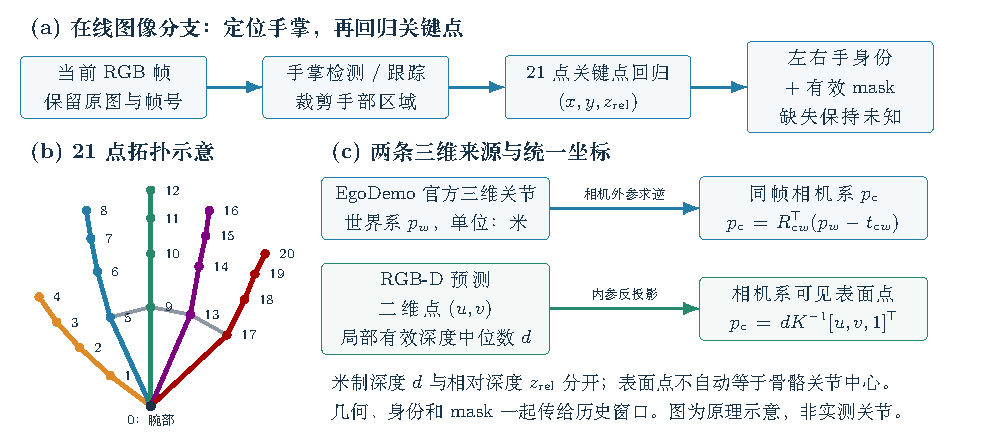
\includegraphics[width=\linewidth]{figures/hand_pose_principle.pdf}
\textbf{上图：}21点估计、五指拓扑与坐标对齐的原理示意。官方世界系姿态与RGB-D在线预测分支分别标注。
\begin{center}
\begin{minipage}{.48\linewidth}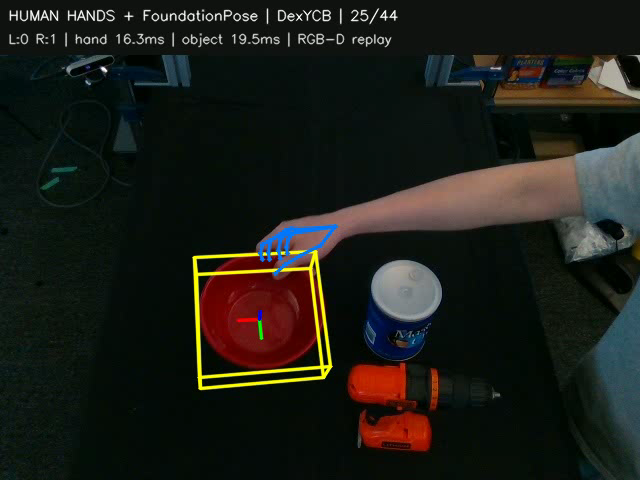
\includegraphics[width=\linewidth]{figures/hand_object_rgbd.png}\end{minipage}\hfill
\begin{minipage}{.48\linewidth}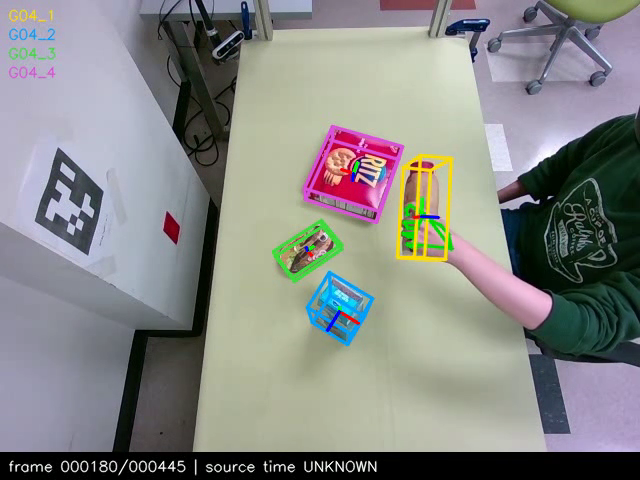
\includegraphics[width=\linewidth]{figures/hocap_four_objects_f180.png}\end{minipage}
\end{center}
\textbf{下图：}真实已有输出。左为DexYCB真人手21点与碗的6D同帧叠加；右为HO-Cap真人场景中的四目标跟踪。颜色框与坐标轴表示物体身份和位姿，不能将叠加效果当作独立精度。
\begin{center}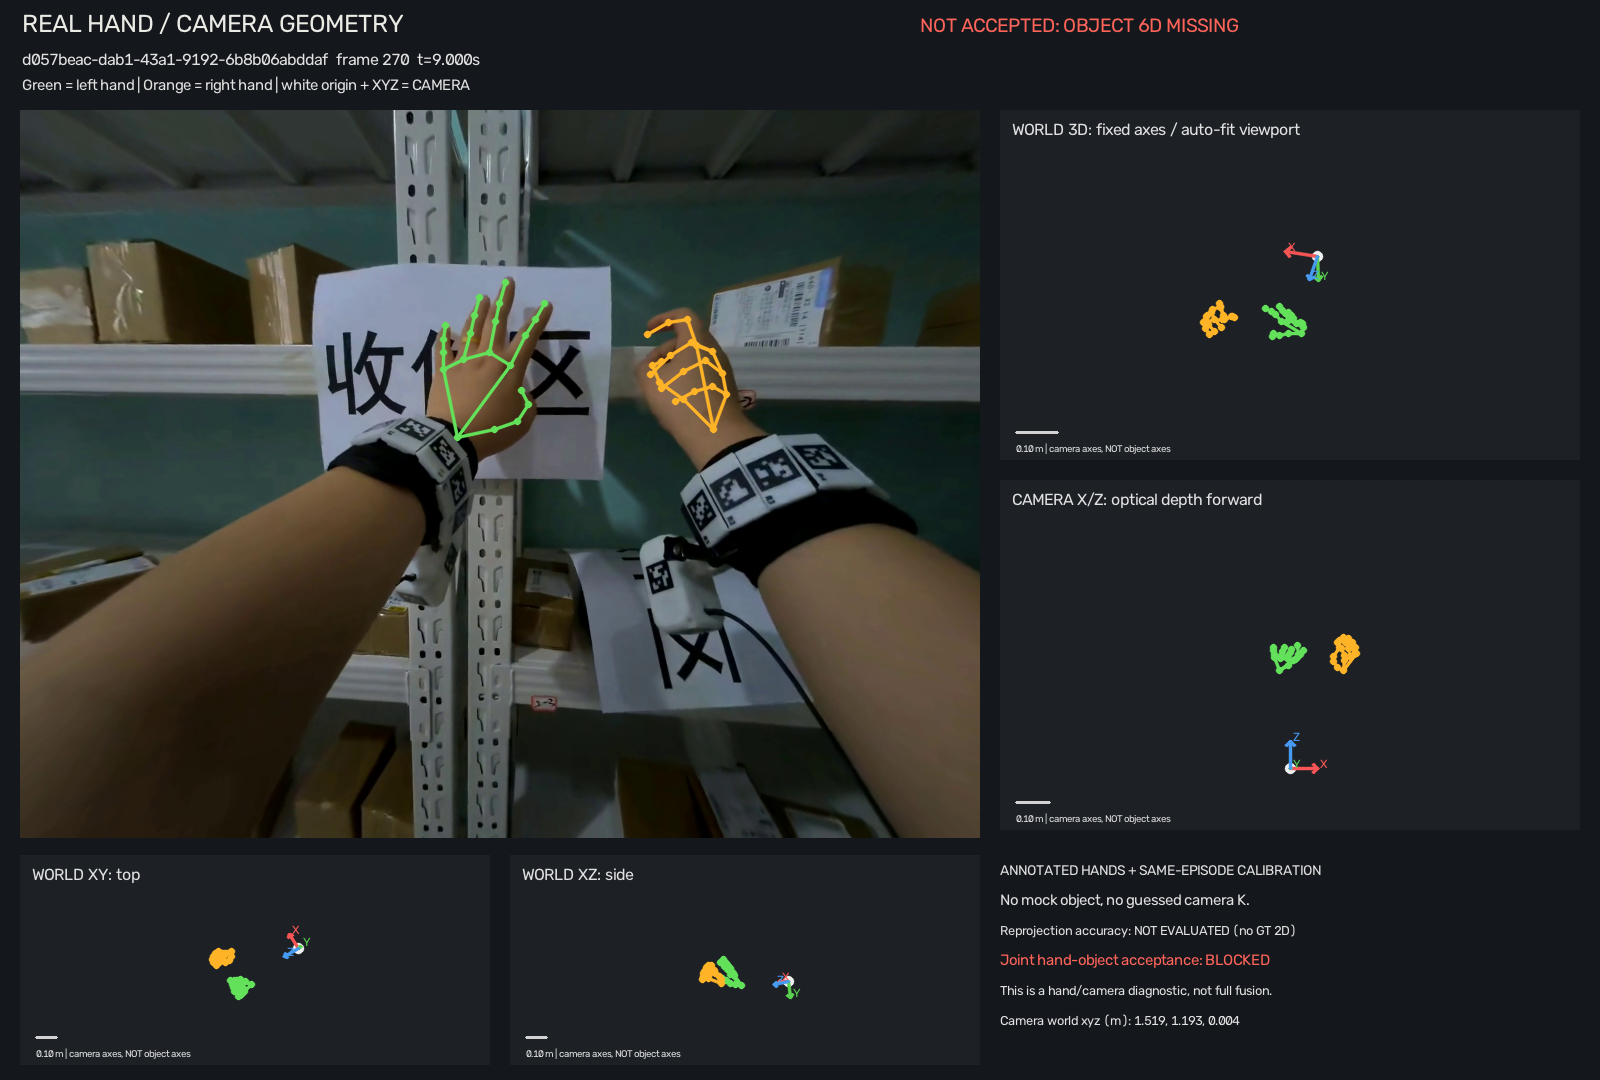
\includegraphics[width=.52\linewidth]{figures/hand_ego_coordinates.png}\end{center}
\small 第一视角官方手关节的相机／世界系投影。此原图为历史手部专项诊断，原画面状态提示保留。

\clearpage
\begin{center}{\Large\bfseries 物体6D：刚体变换与RGB-D跟踪}\end{center}
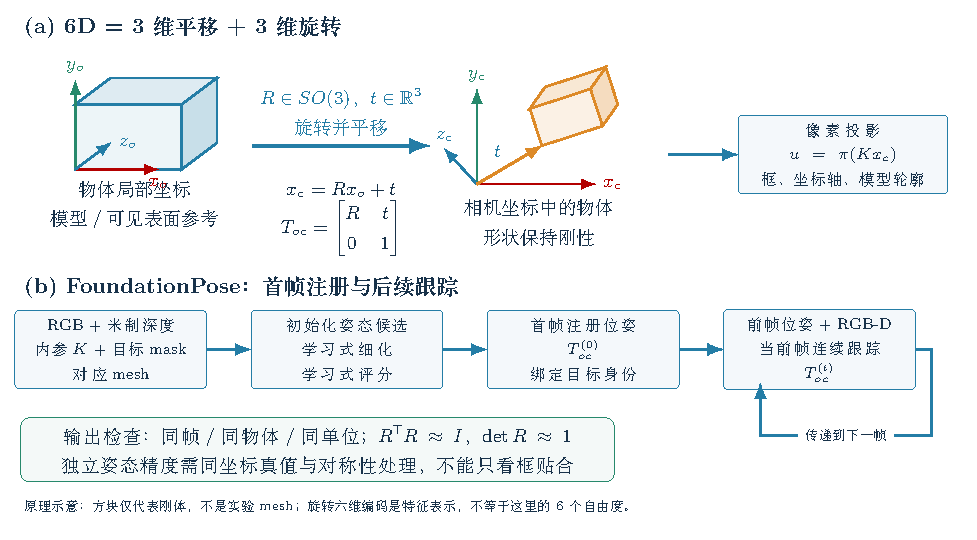
\includegraphics[width=\linewidth]{figures/pose6d_principle.pdf}
\textbf{上图：}三个平移自由度、三个旋转自由度、相机投影，以及FoundationPose首帧注册与后续跟踪。方块和坐标系是原理示意。
\begin{center}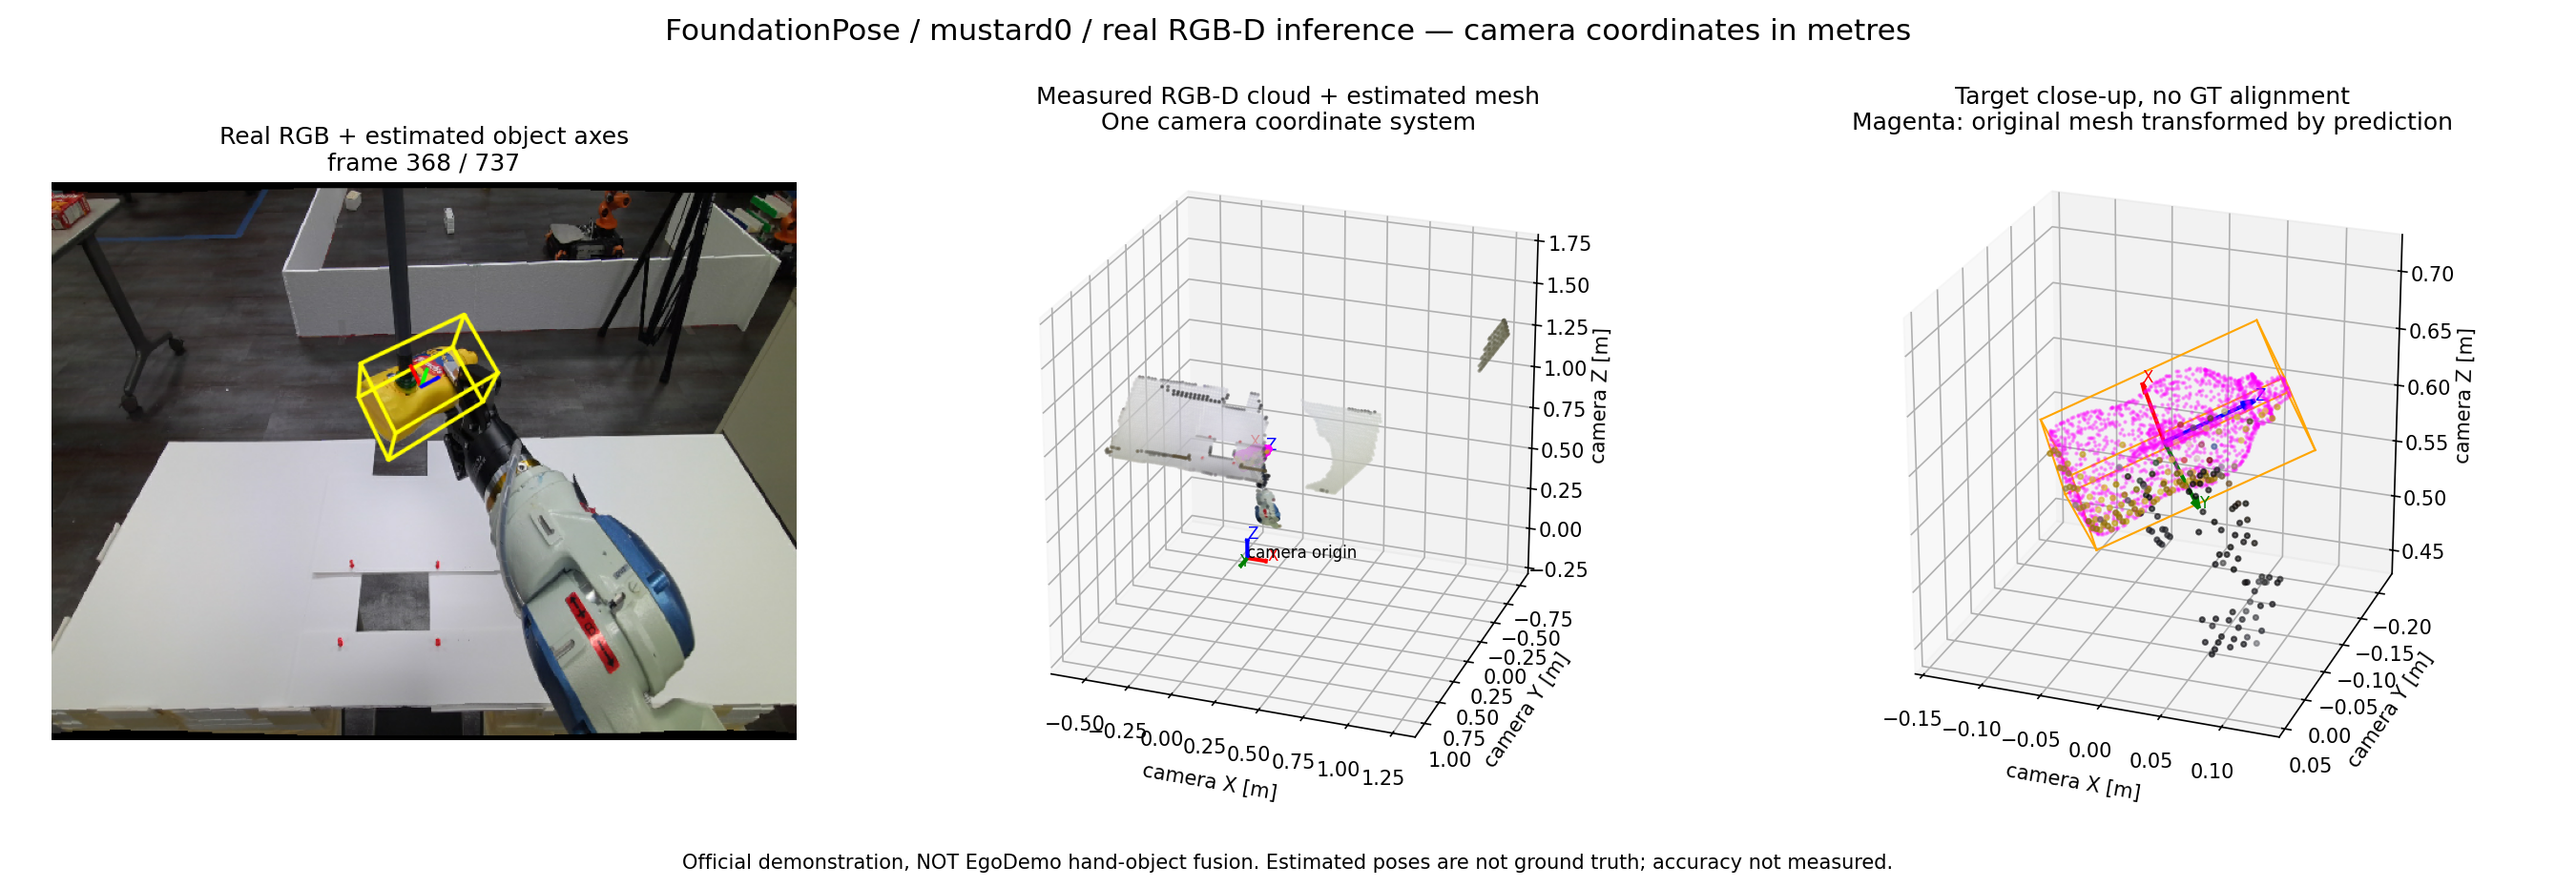
\includegraphics[width=\linewidth]{figures/pose6d_pointcloud.png}\end{center}
\textbf{下图：}真实RGB、深度点云与预测mesh，来自737帧独立后端运行。该场景含机械臂，用于验证6D后端；真人手物示例见第1页。
\begin{center}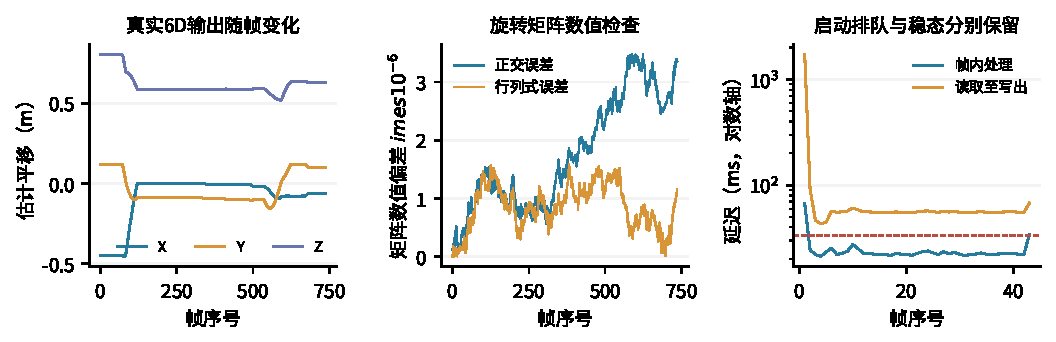
\includegraphics[width=\linewidth]{figures/perception_validation.pdf}\end{center}
\small 指标图依次为位姿平移轨迹、旋转矩阵数值自洽、逐帧时延。轨迹和自洽不是独立真值误差。

\clearpage
\begin{center}{\Large\bfseries 双目重建：同点三角化到表面运动}\end{center}
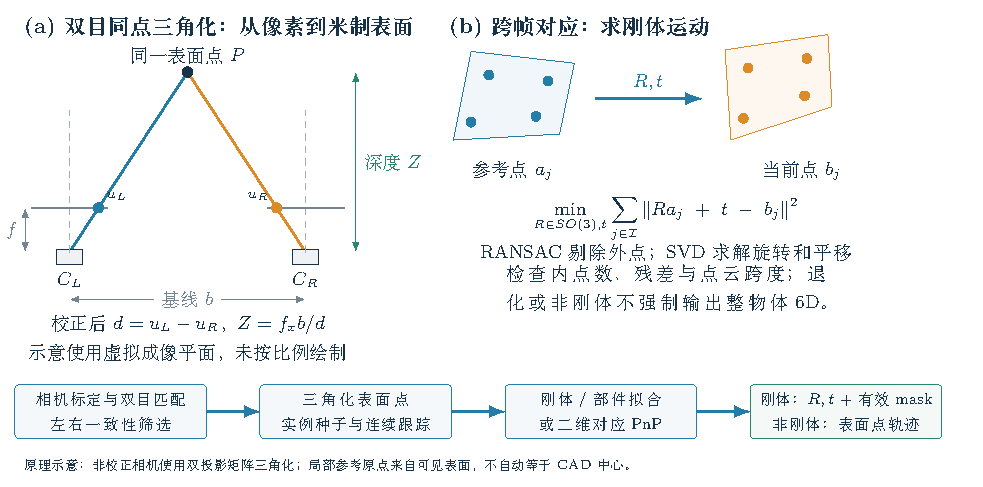
\includegraphics[width=\linewidth]{figures/stereo_geometry_principle.pdf}
\textbf{上图：}基线、视差与深度关系，跨帧对应点的RANSAC／SVD刚体拟合，以及刚体与非刚体的不同输出。
\begin{center}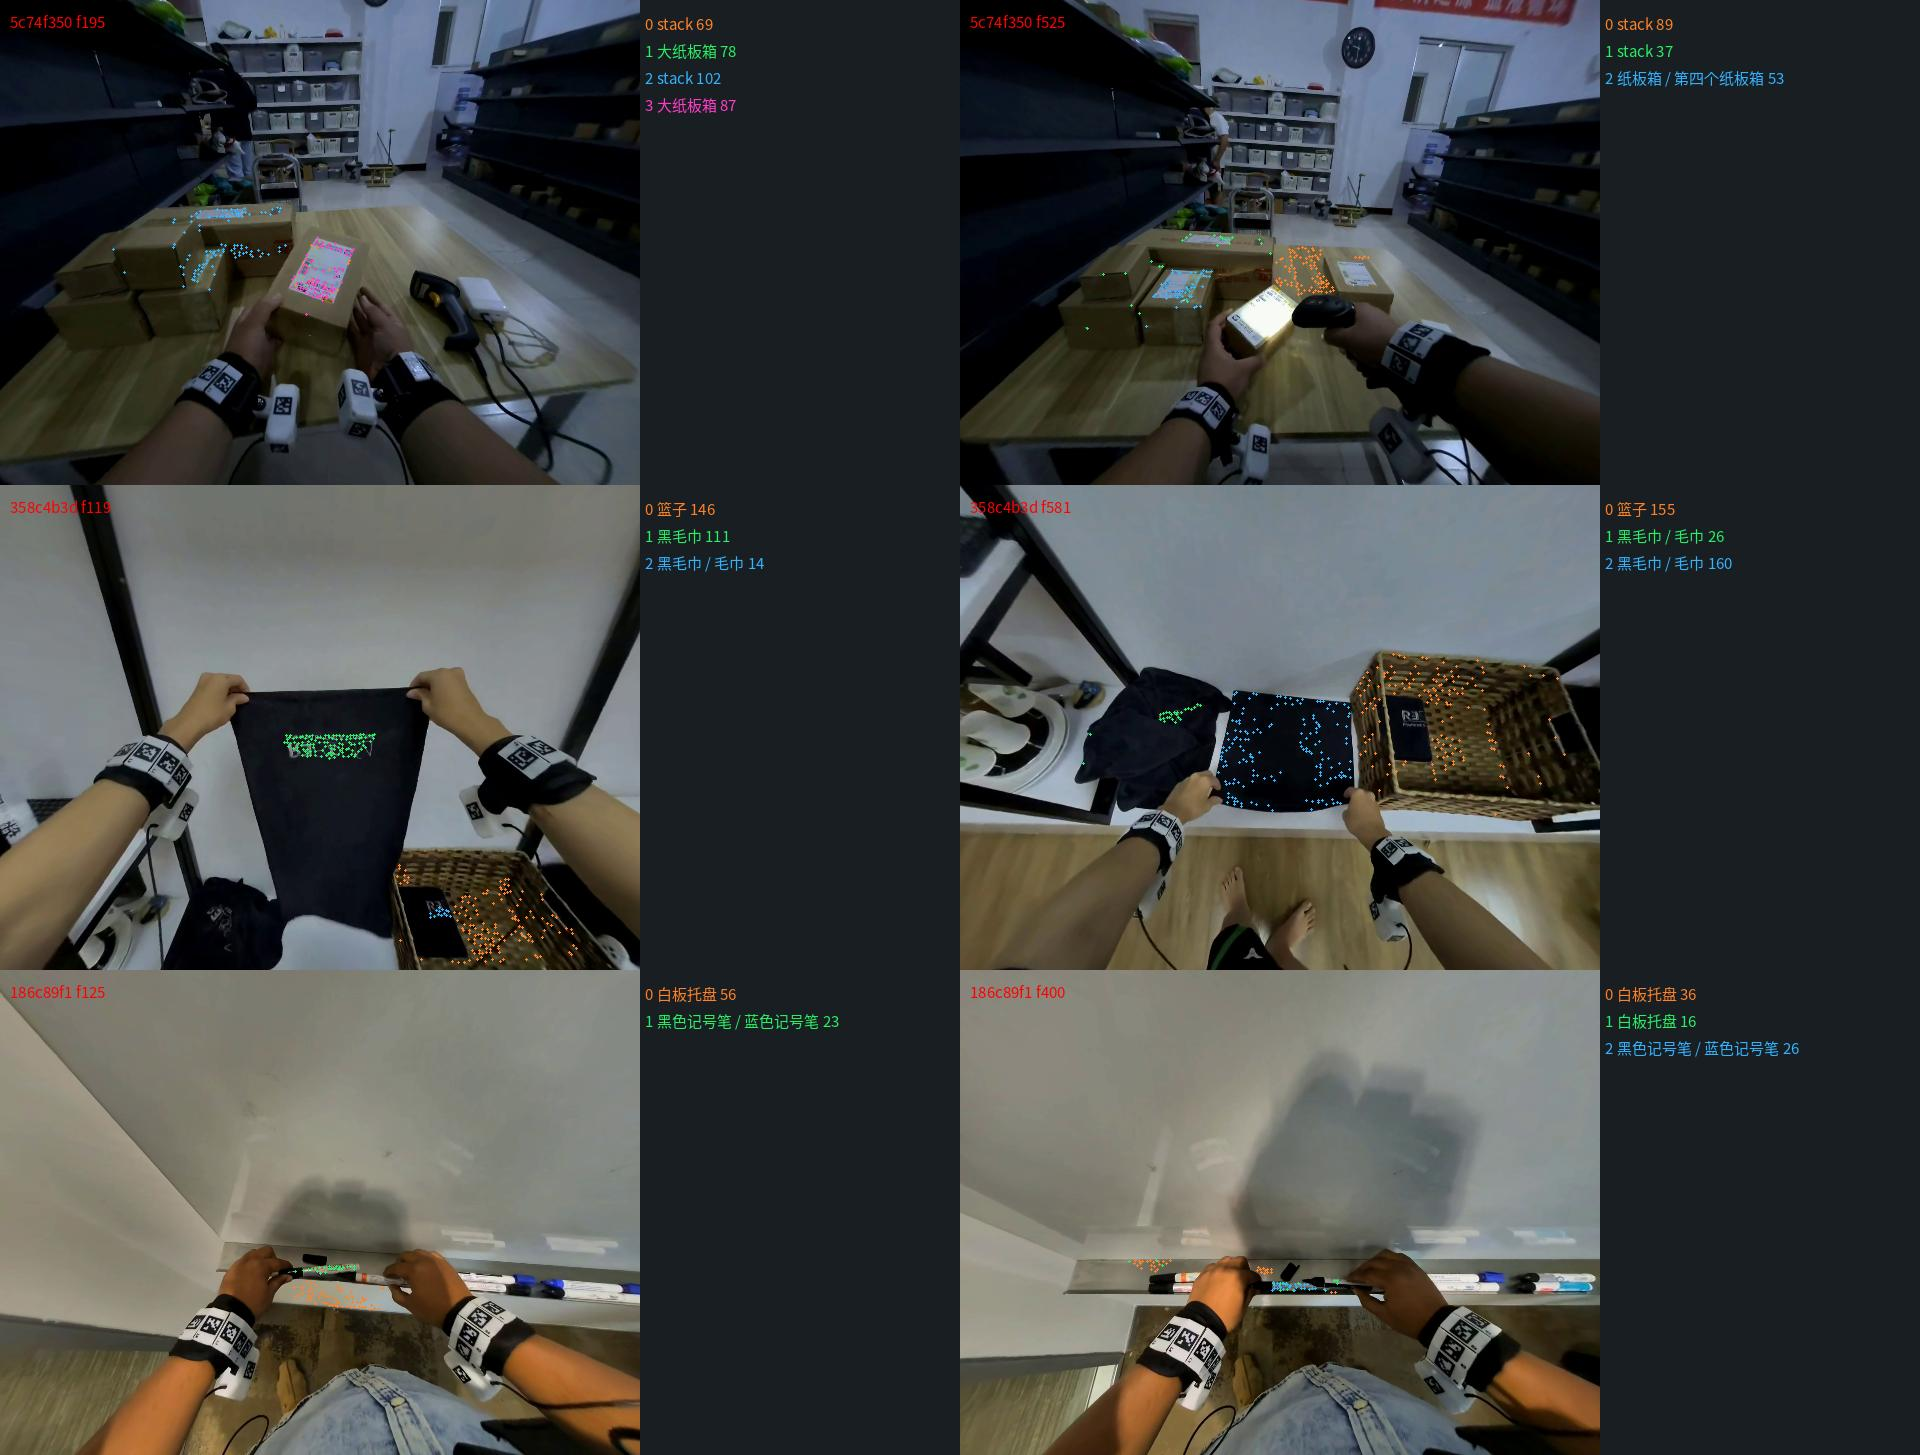
\includegraphics[width=.64\linewidth]{figures/egodemo_surface_seeds.jpg}\end{center}
\textbf{下图：}EgoDemo第一视角的真实表面种子。纸盒、织物和托盘／笔等物体按来源保留表面观测，不把所有表面参考系都视作整物体6D。

这三页为便于直接看图的索引。全部原理图与真实演示也已嵌入\textbf{完整技术报告\_单栏图文版.pdf}正文，图的来源、公式和实测范围以正文为准。
\end{document}
